\section{Durchführung}
\label{sec:Durchfuehrung}
\begin{figure}[H]
    \centering
    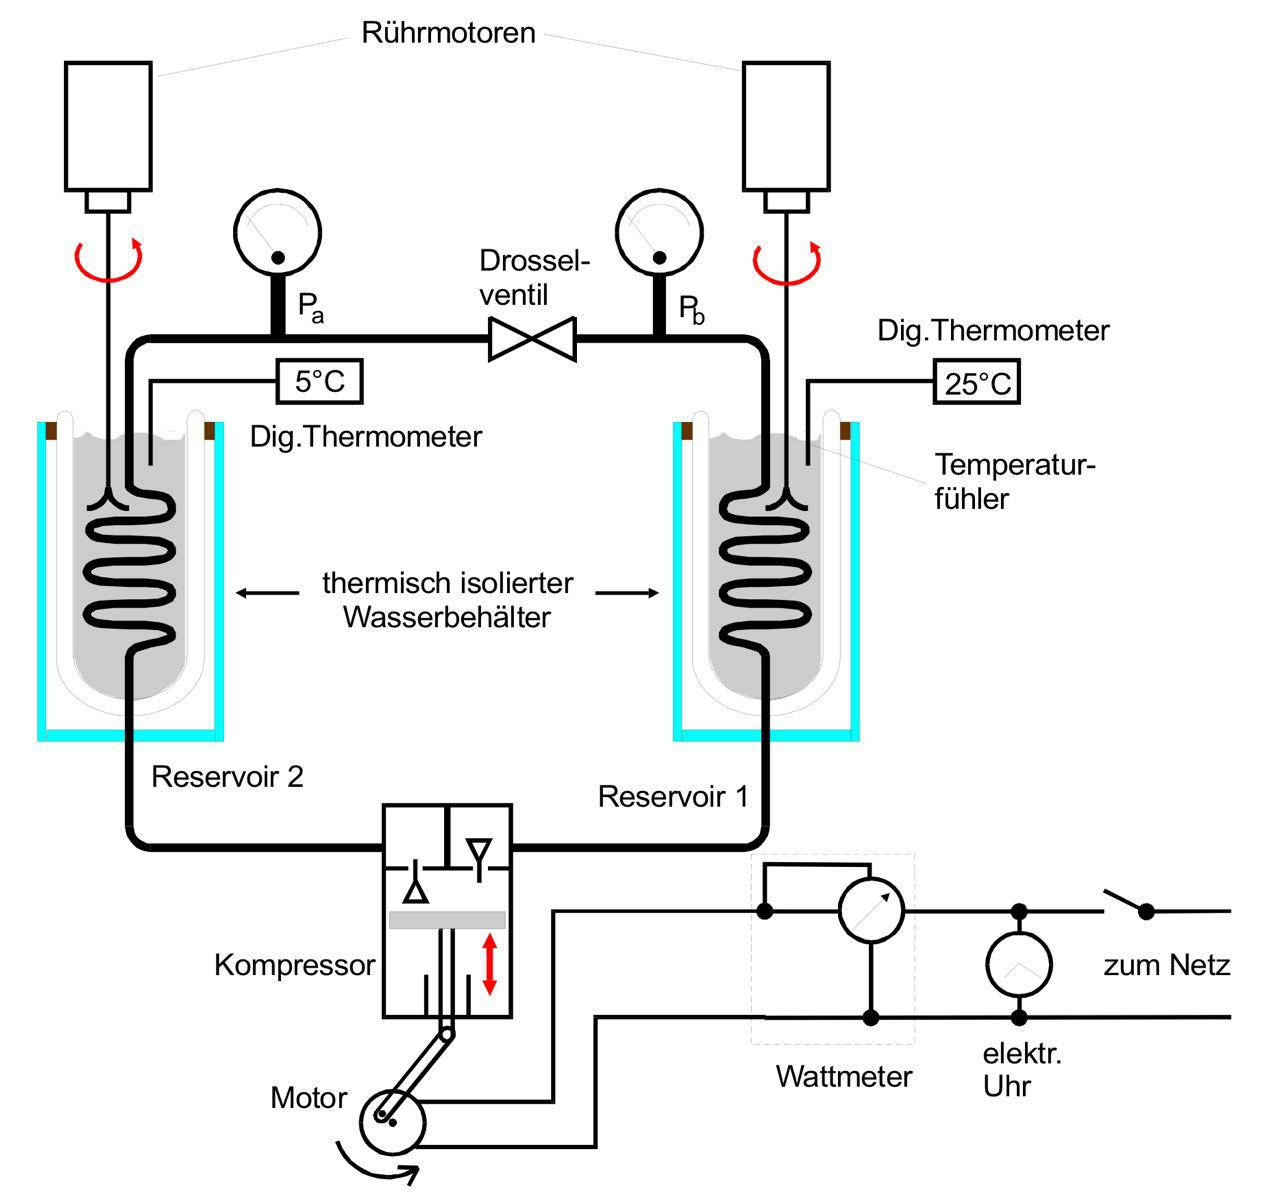
\includegraphics[width=0.5\textwidth]{bilder/aufbau_spezifisch.jpg}
    \caption{Spezifischer Aufbau der Wärmepumpe \cite[197]{Anleitung}}
    \label{fig:aufbau_spezifisch}
\end{figure}

In die Reservoire werden jeweils 3 Liter Wasser gefüllt. Zusätzlich werden
Rührmotore in diese installiert, um eine konstante Temperatur verteilung an 
das Waser zu gewährleisten und ein gefrieren der Leitungen der Wärmepumpe zu verhindern.
Die Reseroire sowie die Leitungen der Wärmepumpe sind dabei wärmeisoliert,
um diese Verluste möglich klein zu halten.\\

Zuerst werden nun die Rührmotoren eingeschaltet und dann die Netzspannung
an den Kompressor angelegt.
Nun wird für jede Minute der Druck $p$ und die Wassertemperatur $T$, sowie die 
Leistung des Kompressors gemessen.